\documentclass{article}
\usepackage[utf8]{inputenc}

\title{\large{\textsc{In-Class Day 15: Graphs and DFS}}}
\date{}

\usepackage{natbib}
\usepackage{graphicx}
\usepackage{amsmath}
\usepackage{amsfonts}
\usepackage{mathtools}
\usepackage{hyperref}
\usepackage[a4paper, portrait, margin=0.8in]{geometry}

\usepackage{listings}


\newcommand\perm[2][n]{\prescript{#1\mkern-2.5mu}{}P_{#2}}
\newcommand\comb[2][n]{\prescript{#1\mkern-0.5mu}{}C_{#2}}
\newcommand*{\field}[1]{\mathbb{#1}}

\DeclarePairedDelimiter\ceil{\lceil}{\rceil}
\DeclarePairedDelimiter\floor{\lfloor}{\rfloor}

\newcommand{\Mod}[1]{\ (\text{mod}\ #1)}

\begin{document}

\maketitle

\subsection*{}


\begin{enumerate}


%%%%% PROBLEM 1 %%%%%
\item Given a directed graph, determine whether or not the graph is also a binary tree.\\
Hint:
This is a valid graph, but not a valid tree.\\
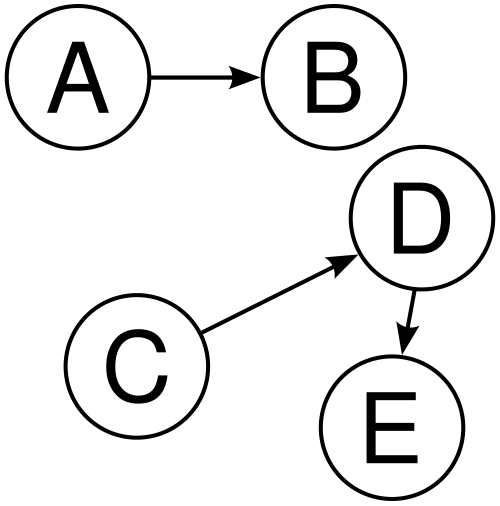
\includegraphics[width=\textwidth/5]{disjointGraph.png}
\\


Assume the following Graph API:

\begin{lstlisting}[language=Java]
void addEdge(int v, int w);
List<Integer> vertices();
int numVertices();
int numEdges();
Iterable<Integer> getNeighbors(int v);
boolean hasEdgeBetween(int v, int w);
\end{lstlisting}


\item You would like to install a piece of software, but you must first install the dependencies of that software before that software can be installed. These dependencies might also have dependencies. For example, in order to install $A$, you might need to install $B$ and $C$ first, but $B$ and $C$ both also need to install $D$ first. Your input will be a list of pairs (in this example, the input would be \texttt{[(A, B), (A, C), (B, D), (C, D)]}). Write an algorithm that will determine in what order to install all the dependencies. In this case, we can install $DBCA$ or $DCBA$. If there are circular dependencies, return \texttt{null}. If $D$ depends on $A$, then this software cannot be installed.

\item You are given a map in the form of a 2-D array. The map will tell whether there exists land (1) or water (0) at that certain spot. Pieces of land are connected if they are adjacent to each other either horizontally or vertically (but not diagonally). Determine how many disjoint islands there are. For example,
\begin{lstlisting}
011100011100000
011100010000000
000111110000010
011000001000000
010100001110000
011100001110000
\end{lstlisting}
represents 4 islands.

\item You are given a combination lock with N-dials, each with M numbers ranging from 1-M. For example, you could have a lock with 4-dials where each dial is a number from 1-7. In each timestep, you can rotate any dial in either direction. For example, a lock currently at 4251 could be set to 5251, 3251, 4351, 4151, 4241, 4261, 4257, or 4252. You are also given a list of blocking combinations. At no time should your combination ever read out any number from the the list of blocking combinations. Given a starting and ending combination and a set of blocking combinations, determine if there is a way to get from the starting combination to the ending combination.
\end{enumerate}

\end{document}
